\chapter{Experiment: hardware system}
This chapter is about the hardware experiment.

ad;falknv.xzfvhlsakjdgfnmdflk asdjgfmndfgb;lkjesf;mngfbl;kjfx.,mszedk.jfal;j

\section{Hardware setup}
This section is about hardware setup and its features.

\begin{figure}[H]
\begin{minipage}[b]{0.45\linewidth}
\centering
\fbox{\includegraphics[width=0.75\linewidth]{figures/double_pendulum_CAD.png}}
\end{minipage}
% Example to add your own logos for Acknowledgment
%\hfill
\begin{minipage}[b]{0.45\linewidth}
\centering
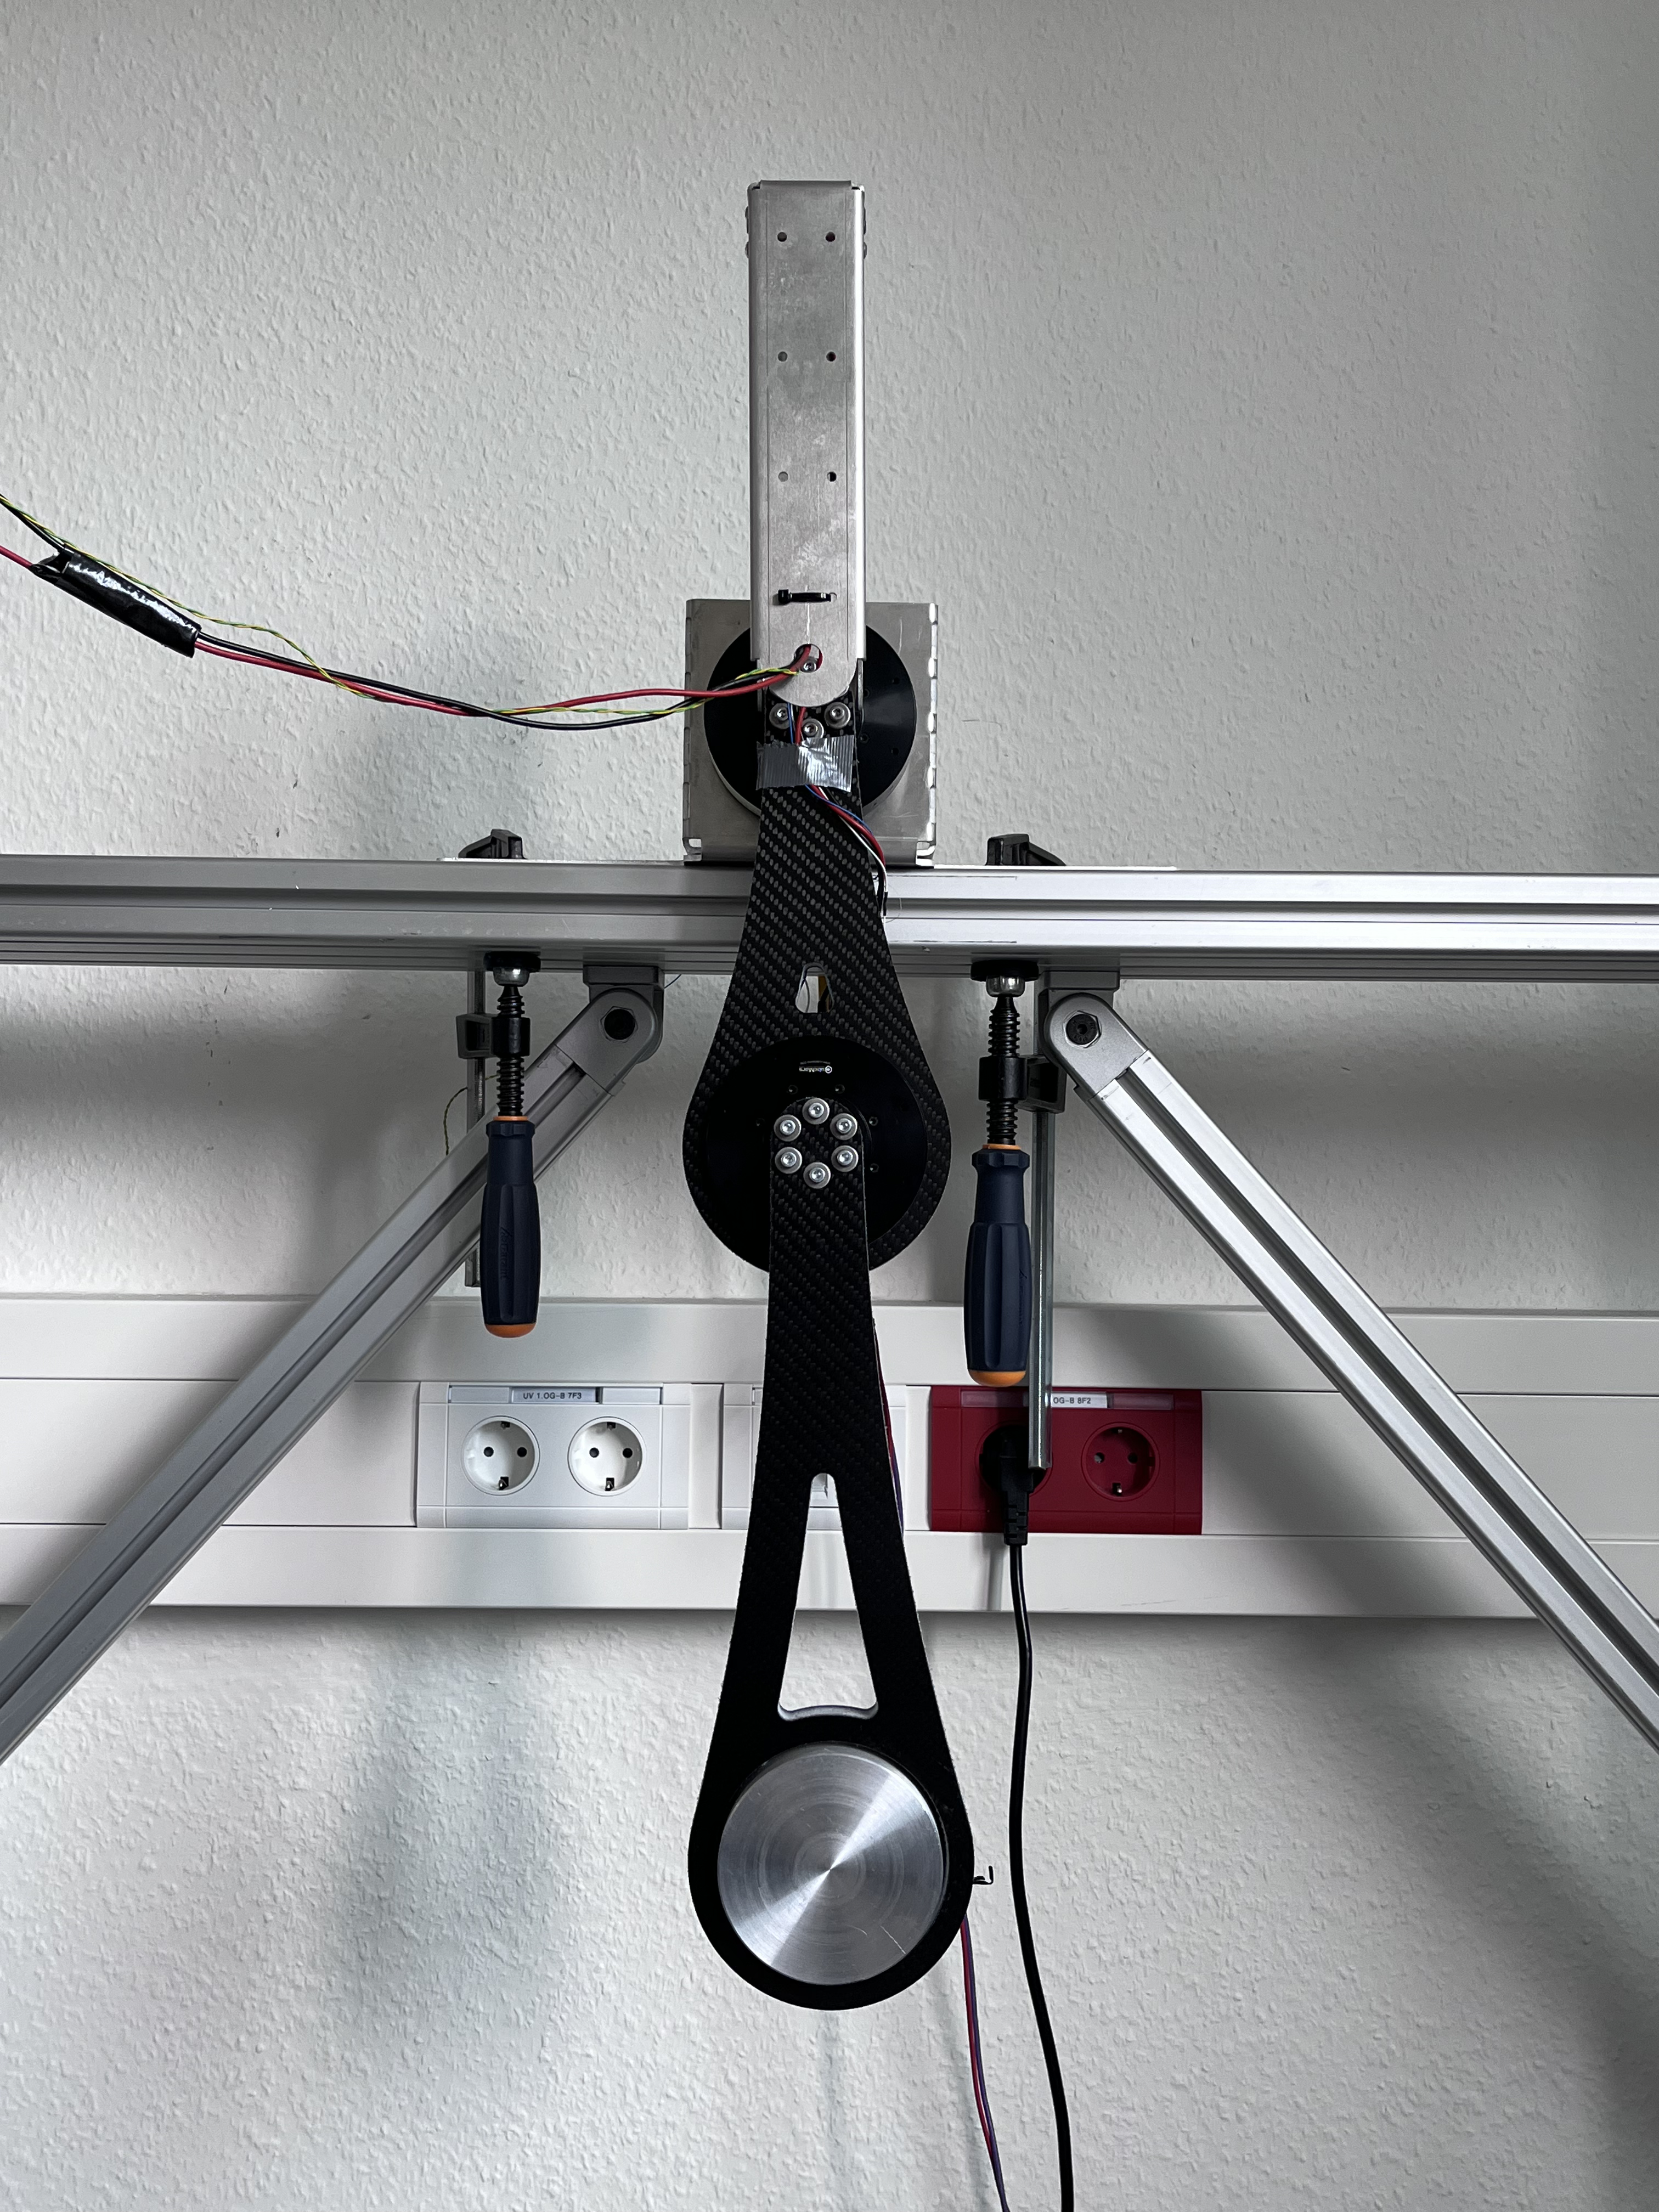
\includegraphics[width=1.0\linewidth]{figures/double_pendulum_real_system.png}
\end{minipage}
\caption{Double pendulum setup in CAD and in real world}
\end{figure}

\begin{figure}[htbp]
  \centering
  \begin{subfigure}[b]{0.45\textwidth}
    \centering
    \includegraphics[width=\textwidth]{figures/hardware_setup/motor.jpg}
    \caption{Figure A}
    \label{fig:subfiga}
  \end{subfigure}
  \hfill
  \begin{subfigure}[b]{0.45\textwidth}
    \centering
    \includegraphics[width=\textwidth]{figures/hardware_setup/torque_speed_curve.jpg}
    \label{fig:subfigb}
    \caption{Figure B}
  \end{subfigure}
  \caption{Two figures side by side}
  \label{fig:twosubfigures}
\end{figure}

\section{system identification}
This section is about the system identification problem when using hardware system.

\section{sim2real problem}
This section is about sim2real problem.

\begin{figure}[htbp]
    \centering
    \fbox{\includegraphics[width=0.9\textwidth]{figures/hardware_result/pendubot_noisy_unclipped.png}} % Second image
    \caption{pendubot noisy simulation result}
    \label{fig:image_b}
\end{figure}






\section{real hardware results}
This section is about simulation results in pendubot and acrobot.

pendubot:

acrobot:

\cleardoublepage
